\hypertarget{main_8cc}{
\section{main.cc File Reference}
\label{main_8cc}\index{main.cc@{main.cc}}
}
Start menu system. 

{\tt \#include \char`\"{}menu.h\char`\"{}}\par


Include dependency graph for main.cc:\nopagebreak
\begin{figure}[H]
\begin{center}
\leavevmode
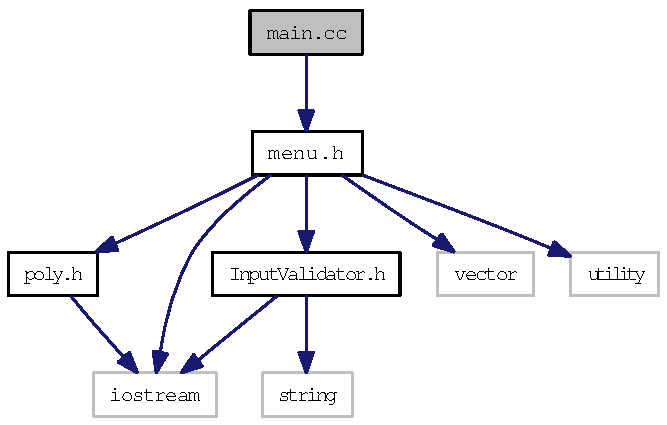
\includegraphics[width=178pt]{main_8cc__incl}
\end{center}
\end{figure}
\subsection*{Functions}
\begin{CompactItemize}
\item 
int \hyperlink{main_8cc_51af30a60f9f02777c6396b8247e356f}{main} ()
\end{CompactItemize}


\subsection{Detailed Description}
Start menu system. 

\begin{Desc}
\item[Author:]Daniel Uber \end{Desc}


Definition in file \hyperlink{main_8cc-source}{main.cc}.

\subsection{Function Documentation}
\hypertarget{main_8cc_51af30a60f9f02777c6396b8247e356f}{
\index{main.cc@{main.cc}!main@{main}}
\index{main@{main}!main.cc@{main.cc}}
\subsubsection[main]{\setlength{\rightskip}{0pt plus 5cm}main ()}}
\label{main_8cc_51af30a60f9f02777c6396b8247e356f}


simple program logic, creates a self starting menu object 

Definition at line 12 of file main.cc.

\begin{Code}\begin{verbatim}12           {
13   PolynomialMenu m;
14   return 0;
15  }
\end{verbatim}
\end{Code}


